
\chapter{Mise en \oe{}uvre de \PpFf}
\label{implementation.chap}


Ce chapitre décrit la fa\c{c}on dont \TT{PpFf} est impl\'ement\'e. 
%
De fa\c{c}on g\'en\'erale, la mise en \oe{}uvre utilise la biblioth\`eque \TT{FastFlow}, et ce en h\'eritant et \'etendant plusieurs de ses classes.

Ce chapitre est divis\'e en deux sections.
%
La premi\`ere section d\'ecrit les diff\'erents éléments composant la biblioth\`eque \TT{PpFf}, et la deuxi\`eme section pr\'esente quelques exemples d\'ecrivant comment un programme \PpFf{} est compil\'e et ex\'ecut\'e.


\section{Les \'el\'ements de \TT{PpFf}}

\GT{Je crois qu'il vaudrait mieux avec la première figure, qui donne
une vrai vue d'ensemble, sans donner trop de détails.  Ensuite, dans
les sous-sections, tu pourras donner la partie de la figure avec les
détails, i.e., les méthodes, etc.}

\IC{Maintenant, je comprends l'idée}

\begin{figure}
\centering
         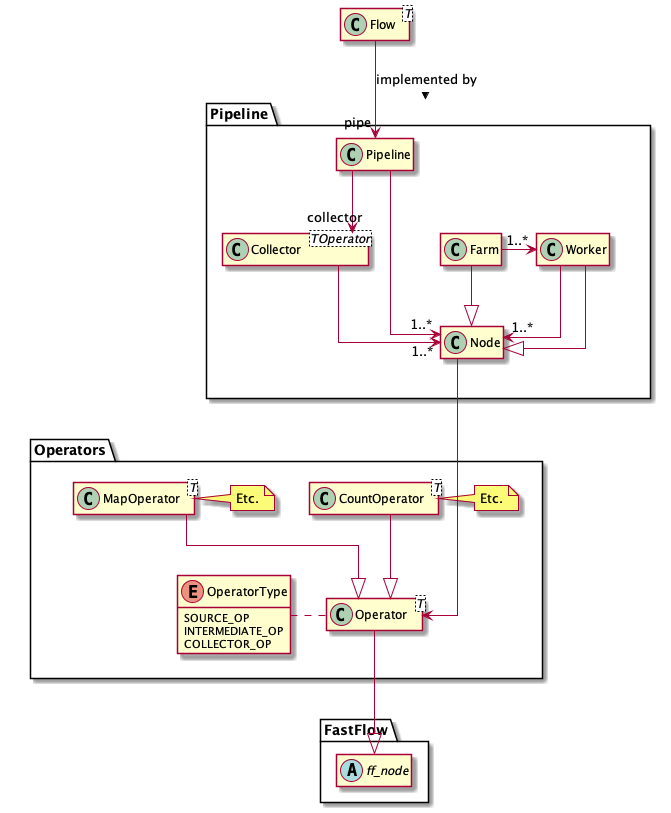
\includegraphics[width=1.0\textwidth]{Figures/vueEnsemble.png}
      \caption{Les principaux éléments (classes) de \TT{PpFf}.}
       \label{All.fig}
\end{figure}

La biblioth\`eque \TT{PpFf} est compos\'ee de plusieurs modules qui permettent de g\'erer les flux de traitement de donn\'ees. Une vue d'ensemble de ces modules est illustr\'ee dans la figure~\ref{All.fig}.

\begin{itemize}

\item Le point d'entr\'ee de \ppff\ est la classe \TT{Flow}, avec laquelle interagissent les d\'eveloppeurs pour cr\'eer des flux de traitement. Toutes les op\'erations de traitement d'un flux de \TT{PpFf} sont li\'ees aux m\'ethodes expos\'ees par cette classe. 

\item Le c\oe{}ur de la mise en \oe{}uvre de \TT{PpFf} est le module \TT{Pipeline}. La cr\'eation et l'ex\'ecution d'un flux sont g\'er\'ees par celui-ci, qui construit tout d'abord une représentation intermédaire, et qui génère ensuite un graphe de n\oe{}uds FastFlow.

\item  Le module \TT{Operators} regroupe tous les op\'erateurs d\'efinis dans \TT{PpFf}. Expos\'es \`a l'utilisateur par le biais de l'\TT{API} de \TT{PpFf}, ces op\'erateurs permettent de traiter les donn\'ees de diverses façons.

\item Le dernier module, \TT{FastFlow}, est la biblioth\`eque au–dessus de laquelle \TT{PpFf} est impl\'ement\'e.


\end{itemize}

\subsection{Flow}

\begin{figure}
\centering
     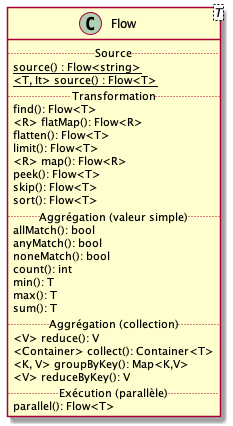
\includegraphics[width=0.5\textwidth]{Figures/flow-details.png}
      \caption{Les diff\'erentes m\'ethodes export\'ees par l'API de \TT{PpFf}.}
       \label{Flow.fig}
\end{figure}



\GT{J'ai modifié le diagramme, pour raffiner la signature générique de
certaines méthodes et \underline{aussi} pour utiliser les mêmes
groupes de méthodes que dans le chapitre précédent --- sinon c'est
mélangeant si deux terminologies/catégorisations différentes sont
utilisées.  Il faudrait donc revoir la partie ci-bas pour utiliser les
mêmes noms de groupe.}

\IC{J'ai révisé la description des groupes selon le nouveau diagramme.}


La classe \TT{Flow} est celle qui définit l'\TT{API} de la biblioth\`eque \TT{PpFf}, l'interface avec laquelle interagit le d\'eveloppeur. La figure~\ref{Flow.fig} --- qui reprend la figure~\ref{MethodesAPI.fig} --- pr\'esente la vue d'ensemble des diverses m\'ethodes export\'ees par \TT{PpFf}. Selon le type export\'e par l'\TT{API}, les m\'ethodes sont divis\'ees en plusieurs groupes : Source, Transformation, Agr\'egation et Ex\'ecution.

Source est le groupe qui permet de d\'efinir un flux de donn\'ees. En g\'en\'eral ce groupe combine les m\'ethodes qui fournissent les donn\'ees au flux. Sans un appel \`a une telle m\'ethode, un flux ne peut pas exister. Le deuxi\`eme groupe du \TT{Flow}, Transformation, est le groupe qui combine les m\'ethodes qui retournent une r\'ef\'erence vers l'objet \TT{Flow}. Ce m\'ecanisme permet d'encha\^iner les m\'ethodes de l'\TT{API}. Le troisi\`eme groupe de \TT{Flow} est le groupe Agr\'egation. Selon le type de r\'esultat produit, ce groupe est-il lui-m\^eme divis\'e en deux sous-cat\'egories : valeur simple qui combine les m\'ethodes retournant une valeur (par ex., r\'esultat bool\'een ou entier) et collection qui combine les m\'ethodes retournant une collection. Dans le dernier groupe de  \TT{Flow}, on retrouve une seule m\'ethode. Cette m\'ethode modifie le comportement d'ex\'ecution du flux. Lorsqu'elle est ajout\'ee dans le  \TT{pipeline}, toutes les op\'erations suivant cette m\'ethode seront ex\'ecut\'ees en parall\`ele en utilisant les instances d'un  \TT{farm}.

L'\TT{API} de \TT{PpFf} permet d'appliquer plusieurs op\'erations les unes à la suite des autres sur une collection de donn\'ees. Ceci est possible en encha\^inant les m\'ethodes (\emph{method chaining}). Les m\'ethodes de l'\TT{API} peuvent \^etre enchain\'ees tant qu'elles retournent une r\'ef\'erence \`a \TT{Flow}. Lorsqu'une m\'ethode retourne une valeur, une valeur simple ou une collection, le traitement est alors ex\'ecut\'e. 


\begin{lstlisting}[
label={count.c++},
language=c++,
gobble=7,
caption={Le code de la m\'ethode \TT{count} de la classe \TT{Flow} de \TT{PpFf}.},
frame=single,
float]
        unsigned int count() {
            typedef CountOperator<int> Count;
            
            pipe.addNodes<Count>(pipe.nbWorkers());
            pipe.run();

            return pipe.value<Count, int>();
        }
\end{lstlisting}

\GT{La méthode est tellement simple que tu es aussi bien de tout
donner son code! Tu peux faire un copier/coller du fichier Flow.hpp,
puis ajouter "gobble" si le code est trop indenté, pour le coller plus
à gauche.}

\IC{Je n'ai pas compris. Est-ce que je dois ajouter toutes les méthodes de Flow ?}


\GT{Puisque tu parles de mise en oeuvre, je crois que tu dois
distinguer entre le flux --- l'objet Flow --- et le pipeline qui met
en oeuvre ce flux, comme indiqué dans le diagramme donnant la vue
d'ensemble --- "implemented by".}

\IC{Merci pour cet explication. Dans ma description, j'ai vu Flow comme étant l'API et Pipeline comme le flux.}

L'\TT{API} de \TT{PpFf} est mise en œuvre par le module \TT{Pipeline}. Ce dernier s'occupe de la cr\'eation et l'ex\'ecution du flux. Le listing~\ref{count.c++} pr\'esente le code de la m\'ethode \TT{count} de l'\TT{API}. L'attribut \TT{pipe} d'un objet \TT{Flow} est une instance de la classe \TT{Pipeline}, objet qui cr\'ee et ajoute les op\'erateurs de type \TT{Count} dans le pipeline associé au flux en appelant la m\'ethode \TT{addNodes}. Une fois les n\oe{}uds ajoutés, puisqu'il s'agit d'une méthode qui produit un résultat qui n'est pas un \TT{Flow}, le traitement associé au pipeline \TT{pipe} est ex\'ecut\'e en appelant la m\'ethode \TT{run}. Puis on obtient et retourne la valeur de type entier (\TT{int}, sp\'ecifi\'e dans le deuxi\`eme param\`etre générique de la m\'ethode \TT{value}) produit par l'exécution du pipeline.

\subsection{Pipeline}
\subsection{Operateurs}


\section{Impl\'ementation de \TT{PpFf} avec \TT{FastFlow} : un exemple}


\begin{itemize}

\item objets1 

\item objets2 

\item objets3 


\end{itemize}
